\section{Evaluation}\label{sec:eval}

In order to evaluate these approaches, the resulting values are normalized to a scale from zero to ten (Equation \ref{math:normalize}, though zero is only the result if the value could not be computed, e.g. when resulting parameters would divide by zero. Additionally, test engineers were conducted and rated different projects using the same scale. Eventually, the euclidean distance (see \autoref{math:euclid_distance})  is used to calculate the distance of each data set in regard to the manually conducted approach.

\begin{equation}
\label{math:normalize}
X^{'} = \frac{X - X_{min}}{X_{max} - X_{min}} * 10
\end{equation}

\begin{equation} 
	\label{math:euclid_distance}
	d(p,q) = \sqrt{\displaystyle\sum_{i=1}^{n} (p_i - q_i)^2}
\end{equation}
	
In total, ten function packages of three projects were evaluated by three different experts. For function IDs, the results for the euclidean distance of each approach to the experts estimation can be seen in \autoref{fig:euclid_distance_fid_result}. For the approach by function groups \autoref{fig:fg_result} shows the results.
The values marked red are the lowest and therefore the closest to the experts reference, while green marks the biggest number, which indicates a large difference in values. For both testing methods (function ID and function group) the Halstead difficulty is performing best with having the smallest euclidean distance in 17 of 20 cases. Cyclomatic complexity showed to be right in the middle between the signal depth analysis (SDA) and the Halstead difficulty.

\begin{figure}[ht]
	\centering
	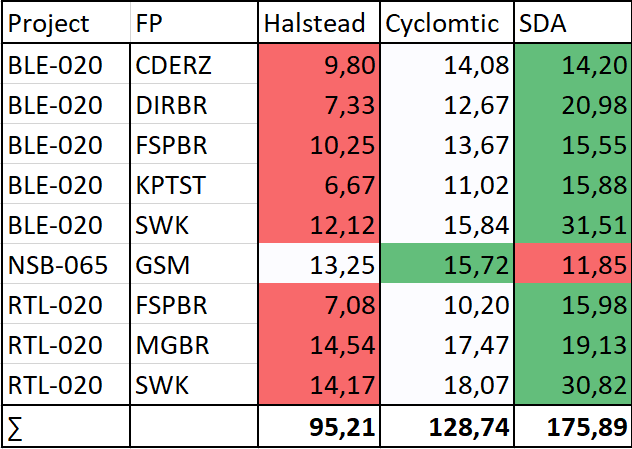
\includegraphics[width=0.7\textwidth]{graphic/FID_RESULT.png}
	\caption{Euclidean distance - Function ID approach} 
	\label{fig:euclid_distance_fid_result}
\end{figure}

\begin{figure}[ht] 
	\centering
	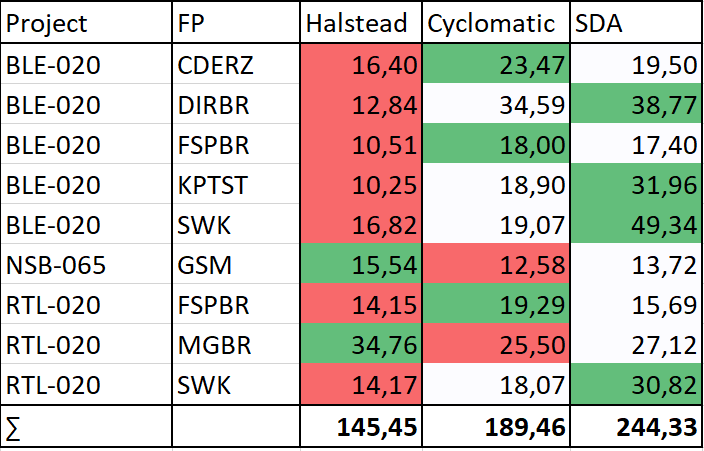
\includegraphics[width=0.7\textwidth]{graphic/FG_RESULT.png}
	\caption{Euclidean distance - Function Group approach}
	\label{fig:fg_result}
\end{figure}

In one case SDA performed best in the function ID approach. In \autoref{fig:plot_gsm_fid} the three examined approaches and the expert evaluation are plotted for NSB 065 - GSM. Function ID 4 is one of the few cases, where the experts evaluation is higher than all approaches. Though when studying all data sets, SDA scores usually the highest overall. This may be one of the reasons, why SDA performed worst in most cases, as the experts rated mostly between two and six. Though all approaches seem to have similar tendencies, since the plots changes mostly in the same directions. It seems the biggest difference between all approaches is the scale. General more complex function packages may be better analyzed by SDA, while more common ones using Halstead.

\begin{figure}[ht]
	\centering
	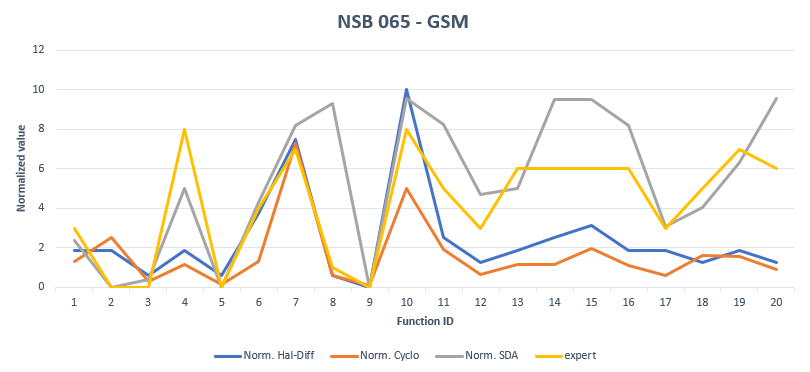
\includegraphics[width=1\textwidth]{graphic/NSB-GSM_plot.png}
	\caption{Complexity comparison NSB - Function ID approach}
	\label{fig:plot_gsm_fid}	
\end{figure}

\begin{figure}[ht] 	
	\centering
	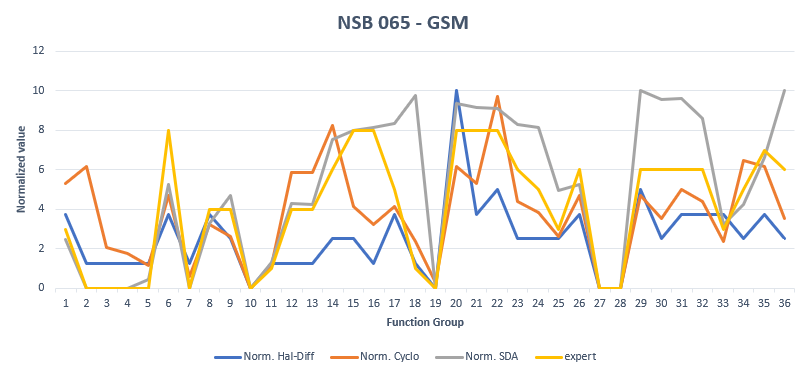
\includegraphics[width=1\textwidth]{graphic/NSB-GSM_FG_plot.png}
	\caption{Complexity comparison NSB - Function Group approach}
	\label{fig:plot_gsm_fg}
\end{figure}

\begin{figure}[ht]
	\centering
	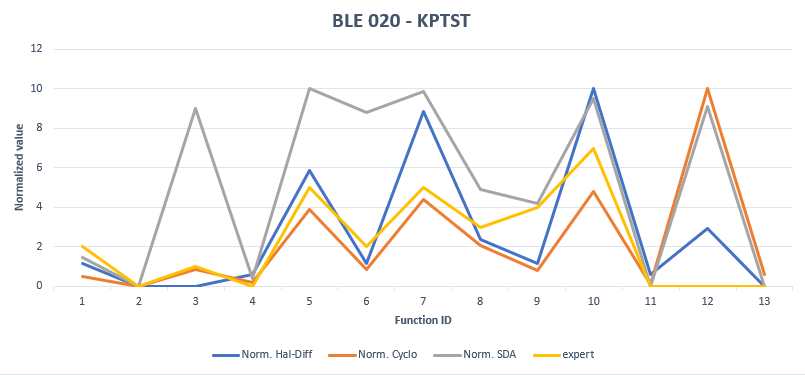
\includegraphics[width=1\textwidth]{graphic/BLE-KPTST_plot.png}	
	\caption{Complexity comparison BLE - Function ID approach}
	\label{fig:plot_ble_fid}
\end{figure}

\begin{figure}[ht]	
	\centering
	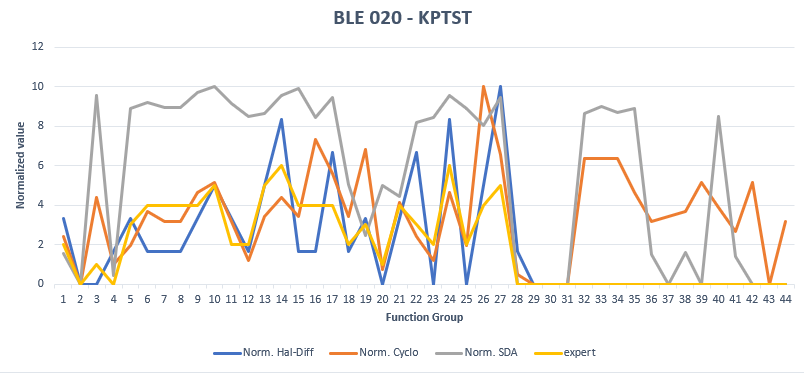
\includegraphics[width=1\textwidth]{graphic/BLE-KPTST_FG_plot.png}
	\caption{Complexity comparison BLE - Function Group approach}
	\label{fig:plot_ble_fg}
\end{figure}